% Font options: 10pm, 11pt, 12pt
% Align headings left instead of center: nocenter
\documentclass[xcolor=x11names,compress]{beamer}\usepackage[]{graphicx}\usepackage[]{color}
%% maxwidth is the original width if it is less than linewidth
%% otherwise use linewidth (to make sure the graphics do not exceed the margin)
\makeatletter
\def\maxwidth{ %
  \ifdim\Gin@nat@width>\linewidth
    \linewidth
  \else
    \Gin@nat@width
  \fi
}
\makeatother

\definecolor{fgcolor}{rgb}{0.345, 0.345, 0.345}
\newcommand{\hlnum}[1]{\textcolor[rgb]{0.686,0.059,0.569}{#1}}%
\newcommand{\hlstr}[1]{\textcolor[rgb]{0.192,0.494,0.8}{#1}}%
\newcommand{\hlcom}[1]{\textcolor[rgb]{0.678,0.584,0.686}{\textit{#1}}}%
\newcommand{\hlopt}[1]{\textcolor[rgb]{0,0,0}{#1}}%
\newcommand{\hlstd}[1]{\textcolor[rgb]{0.345,0.345,0.345}{#1}}%
\newcommand{\hlkwa}[1]{\textcolor[rgb]{0.161,0.373,0.58}{\textbf{#1}}}%
\newcommand{\hlkwb}[1]{\textcolor[rgb]{0.69,0.353,0.396}{#1}}%
\newcommand{\hlkwc}[1]{\textcolor[rgb]{0.333,0.667,0.333}{#1}}%
\newcommand{\hlkwd}[1]{\textcolor[rgb]{0.737,0.353,0.396}{\textbf{#1}}}%
\let\hlipl\hlkwb

\usepackage{framed}
\makeatletter
\newenvironment{kframe}{%
 \def\at@end@of@kframe{}%
 \ifinner\ifhmode%
  \def\at@end@of@kframe{\end{minipage}}%
  \begin{minipage}{\columnwidth}%
 \fi\fi%
 \def\FrameCommand##1{\hskip\@totalleftmargin \hskip-\fboxsep
 \colorbox{shadecolor}{##1}\hskip-\fboxsep
     % There is no \\@totalrightmargin, so:
     \hskip-\linewidth \hskip-\@totalleftmargin \hskip\columnwidth}%
 \MakeFramed {\advance\hsize-\width
   \@totalleftmargin\z@ \linewidth\hsize
   \@setminipage}}%
 {\par\unskip\endMakeFramed%
 \at@end@of@kframe}
\makeatother

\definecolor{shadecolor}{rgb}{.97, .97, .97}
\definecolor{messagecolor}{rgb}{0, 0, 0}
\definecolor{warningcolor}{rgb}{1, 0, 1}
\definecolor{errorcolor}{rgb}{1, 0, 0}
\newenvironment{knitrout}{}{} % an empty environment to be redefined in TeX

\usepackage{alltt}
%\documentclass[xcolor=x11names,compress,handout]{beamer}
\usepackage[]{graphicx}
\usepackage[]{color}
\usepackage{booktabs}
\usepackage{hyperref}
\usepackage{tikz}
\usepackage{multirow}
\usepackage{multicol}
\usepackage{dcolumn}
\usepackage{bigstrut}
\usepackage{amsmath} 
\usepackage{xcolor,colortbl}
\usepackage{amssymb}
%\newcommand{\done}{\cellcolor{teal}#1}

%% Beamer Layout %%%%%%%%%%%%%%%%%%%%%%%%%%%%%%%%%%
\useoutertheme[subsection=false,shadow]{miniframes}
\useinnertheme{default}
\usefonttheme{serif}
\usepackage{Arev}
\usepackage{pdfpages}

\setbeamerfont{title like}{shape=\scshape}
\setbeamerfont{frametitle}{shape=\scshape, size=\normalsize}

\definecolor{dkblue}{RGB}{0,0,102}

\setbeamercolor*{lower separation line head}{bg=dkblue} 
\setbeamercolor*{normal text}{fg=black,bg=white} 
\setbeamercolor*{alerted text}{fg=red} 
\setbeamercolor*{example text}{fg=black} 
\setbeamercolor*{structure}{fg=black} 
 
\setbeamercolor*{palette tertiary}{fg=black,bg=black!10} 
\setbeamercolor*{palette quaternary}{fg=black,bg=black!10} 

\renewcommand{\(}{\begin{columns}}
\renewcommand{\)}{\end{columns}}
\newcommand{\<}[1]{\begin{column}{#1}}
\renewcommand{\>}{\end{column}}

\setbeamertemplate{navigation symbols}{} 
\setbeamertemplate{footline}[frame number]
\setbeamertemplate{caption}{\raggedright\insertcaption\par}

\setbeamersize{text margin left=5pt,text margin right=5pt}

\AtBeginSection{\frame{\sectionpage}}
\usepackage{xcolor}
\hypersetup{
    colorlinks,
    linkcolor={red!50!black},
    citecolor={blue!50!black},
    urlcolor={blue!80!black}
}

\setbeamercolor{block title}{use=structure,fg=white,bg=structure.fg!75!orange}
\setbeamercolor{block body}{parent=normal text,use=block title,bg=block title.bg!10!bg}

%%%%%%%%%%%%%%%%%%%%%%%%%%%%%%%%%%%%%%%%%%%%%%%%%%



\title{FLS 6441 - Methods III: Explanation and Causation}
\subtitle{Week 5 - Natural Experiments}
\author{Jonathan Phillips}
\date{April 2019}
\IfFileExists{upquote.sty}{\usepackage{upquote}}{}
\begin{document}  

\frame{\titlepage}

\begin{frame}
\frametitle{Classification of Research Designs}
\footnotesize
\begin{table}[htbp]
  \centering
    \begin{tabular}{|p{2.9cm}|p{2.5cm}|p{2.5cm}|}
    \hline
          & \multicolumn{1}{p{2.9cm}|}{\textbf{Independence of Treatment Assignment?}} & \multicolumn{1}{p{2.5cm}|}{\textbf{Researcher Controls Treatment Assignment?}} \bigstrut\\
    \hline
    \textbf{Controlled Experiments} & \checkmark      & \checkmark  \bigstrut\\
    \hline
    \textbf{Natural Experiments} & \checkmark      &  \bigstrut\\
    \hline
    \textbf{Observational Studies} &       &  \bigstrut\\
    \hline
    \end{tabular}%
  \label{tab:addlabel}%
\end{table}%
\normalsize
\end{frame}


\begin{frame}
\frametitle{Classification of Research Designs}
\footnotesize
\begin{table}[htbp]
  \centering
  \scalebox{0.7}{
    \begin{tabular}{|p{2.2cm}|p{5cm}|c|c|}
    \hline
          &       & \multicolumn{1}{p{2.4cm}|}{\textbf{Independence of Treatment Assignment}} & \multicolumn{1}{p{3cm}|}{\textbf{Researcher Controls Treatment Assignment?}} \bigstrut\\
    \hline
    \multicolumn{1}{|p{2.9cm}|}{\multirow{2}[4]{2.9cm}{\textbf{Controlled Experiments}}} & Field Experiments & \checkmark      & \checkmark  \bigstrut\\
\cline{2-4}          & Survey and Lab Experiments &  \checkmark     & \checkmark \bigstrut\\
    \hline
          &       &       &  \bigstrut\\
    \hline
    \multicolumn{1}{|p{2.9cm}|}{\multirow{3}[6]{2.9cm}{\textbf{Natural Experiments}}} & Natural Experiments &  \checkmark     &  \bigstrut\\
\cline{2-4}          & Instrumental Variables & \checkmark      &  \bigstrut\\
\cline{2-4}          & Discontinuities & \checkmark      &  \bigstrut\\
    \hline
          &       &       &  \bigstrut\\
    \hline
    \multicolumn{1}{|p{2.9cm}|}{\multirow{4}[8]{2.9cm}{\textbf{Observational Studies}}} & Difference-in-Differences &       &  \bigstrut\\
\cline{2-4}          & Controlling for Confounding &       &  \bigstrut\\
\cline{2-4}          & Matching &       &  \bigstrut\\
\cline{2-4}          & Comparative Cases and Process Tracing &       &  \bigstrut\\
    \hline
    \end{tabular}}%
  \label{tab:addlabel}%
\end{table}%
\normalsize
\end{frame}

\section{Natural Experiments}

\begin{frame}
\frametitle{Natural Experiments}
\begin{multicols}{2}
\textbf{Advantages:}
\begin{itemize}
\item We don't need to run our own experiment! (Too expensive, unethical or politically impossible)
\pause
\item Still have independence of potential outcomes from treatment
\pause
\item Treatment may be more 'realistic' than in a controlled experiment
\pause
\end{itemize}
\columnbreak
\textbf{Disadvantages:}
\begin{itemize}
\item We can never be sure randomization really worked
\pause
\item We don't get to choose the treatments we want to evaluate, just 'discover' them
\pause
\item We don't get to choose the population and sample
\end{itemize}
\end{multicols}
\end{frame}

\begin{frame}
\frametitle{Verifying Randomization}
\begin{itemize}
\item If it's an important treatment, \textit{someone} had an incentive to try and alter it
\pause
\item The burden of proof is on us: How can we increase confidence that assignment was (as-if) random?
\pause
\item Two strategies:
\pause
\begin{enumerate}
\item Check balance on lots of variables
\begin{itemize}
\item Especially variables that are potential omitted variables
\end{itemize}
\pause
\item \textbf{Causal Process Observations}
\pause
\begin{itemize}
\item Documents/code/video evidence
\pause
\item Interviews with eyewitnesses
\pause
\item Verifying treatment assignment matches documents
\pause
\item Identify risks of reverse causation, omitted variables, (Self-)selection
\end{itemize}
\end{enumerate}
\end{itemize}
\end{frame}

\begin{frame}
\frametitle{Verifying Randomization}
\begin{itemize}
\item How does Snow argue that households' assignment to water company is as-if random?
\pause
\item How do we know that Brazil's municipal audits are random?
\end{itemize}
\end{frame}

%[Ask about Snow example of water companies - how worked out treatment assignment independent of POs]

\begin{frame}
\frametitle{The Problem of Not Controlling Treatment Assignment}
\begin{itemize}
\item ``Random assignment of the intervention is not sufficient to provide an unbiased estimate of the causal effect.'' (Sekhon and Titunik 2012)
\pause
\item Treatment and control groups are defined \textit{after} randomization - it's our responsibility to make sure:
\pause
\begin{enumerate}
\item \textbf{These two groups actually are comparable} (POs are independent of treatment)
\pause
\begin{itemize}
\item We can only compare those units \textit{that were part of the original randomization}
\end{itemize}
\pause
\item \tetbf{That the treatment is the factor we actually want to study}
\pause
\begin{itemize}
\item We have to 'interpret' the treatment
\pause
\item Sometimes treatments are 'bundles'
\pause
\item Sometimes treatments are 'repeated', creating interactions or changing expectations
\end{itemize}
\end{enumerate}
\end{itemize}
\end{frame}

\begin{frame}
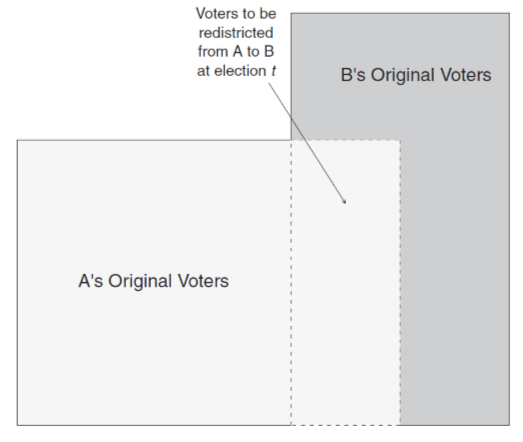
\includegraphics[scale=0.36]{Sekhon_redistricting_a.png}
\end{frame}

\begin{frame}
\frametitle{The Problem of Not Controlling Treatment Assignment}
\footnotesize
\begin{table}[htbp]
  \centering
    \begin{tabular}{|p{3cm}|p{2.4cm}|p{2.4cm}|p{2.4cm}|}
    \hline
          & \textbf{A's Original Voters} & \textbf{Switched Voters} & \multicolumn{1}{p{2.4cm}}{\textbf{B's Original Voters}} \bigstrut\\
    \hline
    2000 election context &       & \cellcolor[rgb]{ .776,  .878,  .706}Same  & \cellcolor[rgb]{ .776,  .878,  .706}\multicolumn{1}{p{2.4cm}}{Same} \bigstrut\\
    \hline
    Duration of exposure to incumbent in district B &       & 4 years & \multicolumn{1}{p{2.4cm}}{10 years} \bigstrut\\
    \hline
    1996 and prior election context & \cellcolor[rgb]{ .776,  .878,  .706}Same  & \cellcolor[rgb]{ .776,  .878,  .706}Same  &  \bigstrut\\
    \hline
    \end{tabular}%
  \label{tab:addlabel}%
\end{table}
\normalsize
\end{frame}

\begin{frame}
\frametitle{The Problem of Not Controlling Treatment Assignment}
\footnotesize
\begin{table}[htbp]
  \centering
    \begin{tabular}{|p{3.2cm}|p{2.6cm}|p{2.6cm}|}
    \hline
          & \textbf{A's Original Voters vs. Switched Voters} & \textbf{B's Original Voters vs. Switched Voters} \bigstrut\\
    \hline
    Potential Outcomes Independent of Treatment Assignment? & \multicolumn{1}{c|}{\cellcolor[rgb]{ .776,  .878,  .706} Yes} & \multicolumn{1}{c|}{No} \bigstrut\\
    \hline
    What is 'Treatment'? & Different election context, different candidates & \cellcolor[rgb]{ .776,  .878,  .706} Difference in duration of exposure to incumbent \bigstrut\\
    \hline
    \end{tabular}%
  \label{tab:addlabel}%
\end{table}%
\normalsize
\end{frame}


\section{Randomized Natural Experiments}

\begin{frame}
\frametitle{Ferraz and Finan (2008)}
\begin{itemize}
\item Do voters punish corrupt politicians?
\pause
\item Corruption is hard to manipulate (ethically)
\pause
\item We can also look at voters' \textit{information} about corruption 
\end{itemize}
\end{frame}

\begin{frame}
\frametitle{Ferraz and Finan (2008)}
\begin{itemize}
\item \textbf{Population:} Brazilian municipalities with population less than 450,000
\item \textbf{Sample:} 373 Municipalities with audits either side of 2004 elections and first-term mayors
\item \textbf{Treatment:} CGU Audit before election
\item \textbf{Control:} Audit after election
\item \textbf{Treatment Assignment Mechanism:} Randomized (Caixa)
\item \textbf{Outcome:} Vote Share for the Incumbent
\end{itemize}
\end{frame}

\begin{frame}
\frametitle{Ferraz and Finan (2008)}
\begin{itemize}
\item Methodology
\begin{itemize}
\item $VS_{ms} = \alpha + \beta \text{Audited Early}_{ms} + X_{ms} + FE_{s} + \epsilon_{ms}$
\pause
\item Result: No Effect
\end{itemize}
\end{itemize}
\end{frame}

\begin{frame}
\frametitle{Ferraz and Finan (2008)}
\begin{itemize}
\item The importance of a theoretical model:
\pause
\item Treatment is the release of information, but the \textit{theory} they seek to test is when voters learn something about candidates 
\pause
\item So we need treatment and control groups reflecting the theory
\pause
\item Voters'\textit{priors} about the candidate's corruption vary
\pause
\item And the \textit{content} of the information varies
\pause
\item It's the interaction of expectations and information content that matters
\end{itemize}
\end{frame}

\begin{frame}
\frametitle{Ferraz and Finan (2008)}
\begin{itemize}
\item Methodology
\begin{itemize}
\item So expected results are \textit{conditional on content of the audit report}
\pause
\item $VS_{ms} = \alpha + \beta \text{Audited Early}_{ms} + \beta_2 \text{Corruption}_{ms} + \beta_3 \text{Audited Early}_{ms}*\text{Corruption}_{ms} + X_{ms} + \text{FE}_{s} + \epsilon_{ms}$
\end{itemize}
\end{itemize}
\end{frame}

\begin{frame}
\frametitle{Ferraz and Finan (2008)}
\begin{itemize}
\item Results
\pause
\begin{itemize}
\item Strong corruption information (2 violations) reduces re-election by 7\% points
\pause
\item Stronger corruption information (3 violations) reduces re-election by 14\% points
\pause
\item Strong corruption information (2 violations) with local radio reduces re-election by 11\% points
\end{itemize}
\end{itemize}
\end{frame}

\begin{frame}
\begin{center}
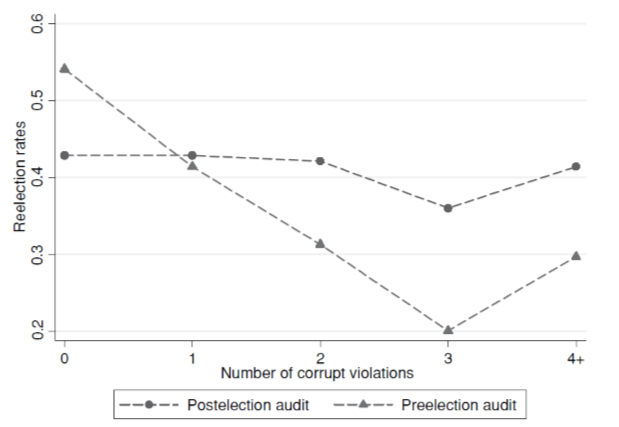
\includegraphics[scale=0.45]{Chart_FF.png}
\end{center}
\end{frame}

\section{Non-Randomized Natural Experiments}

\begin{frame}
\frametitle{Non-Randomized Natural Experiments}
\begin{itemize}
\item How can we achieve causal inference without randomization?
\pause
\item Our assumption is always "The Treatment Assignment Mechanism is independent of potential outcomes"
\pause
\item Can we find real-world treatment assignments that ignored potential outcomes?
\begin{itemize}
\pause
\item "As good as random", "As-if random"
\end{itemize}
\end{itemize}
\end{frame}

\begin{frame}
\frametitle{Non-Randomized Natural Experiments}
\begin{itemize}
\item There are good reasons to be skeptical: Humans are \textit{strategic} and anticipate potential outcomes 
\pause
\item But sometimes they are trying to alter outcomes \textit{different to the potential outcomes we care about}
\pause
\begin{itemize}
\item If these outcomes are not correlated with (/'orthogonal to'/'independent of') our own potential outcomes, we might be okay
\pause
\item But we cannot test this
\pause
\item We have to rely on qualitative evidence of the treatment assignment mechanism
\end{itemize}
\end{itemize}
\end{frame}

\begin{frame}
\frametitle{Posner (2004)}
\begin{itemize}
\item \textbf{Hypothesis:} Cultural differences become political cleavages when the cultural groups are large portions of the population
\pause
\item \textbf{Treatment: } Smaller country (relative to size of ethnic group)
\pause
\item \textbf{Control: } Larger country
\pause
\item \textbf{Potential Outcomes:} Degree of political conflict between ethnic groups in larger/smaller countries
\pause
\item \textbf{Treatment Assignment Mechanism:} African borders that cross ethnic group boundaries
\end{itemize}
\end{frame}

\begin{frame}
\frametitle{Posner (2004)}
\begin{itemize}
\item African colonial borders assigned people to be 'Zambian' or 'Malawian'. 
\pause
\item Straight lines drawn with a ruler in Berlin
\pause
\item Little knowledge of local geography or populations
\pause
\item Zambia-Malawi border defined by geography: by the watershed of the hills
\pause
\item Splitting the Chewa and Tumbuka groups
\end{itemize}
\end{frame}

\begin{frame}
\includegraphics[width=0.8\textwidth]{Arbitrary_borders.jpg}
\end{frame}

\begin{frame}
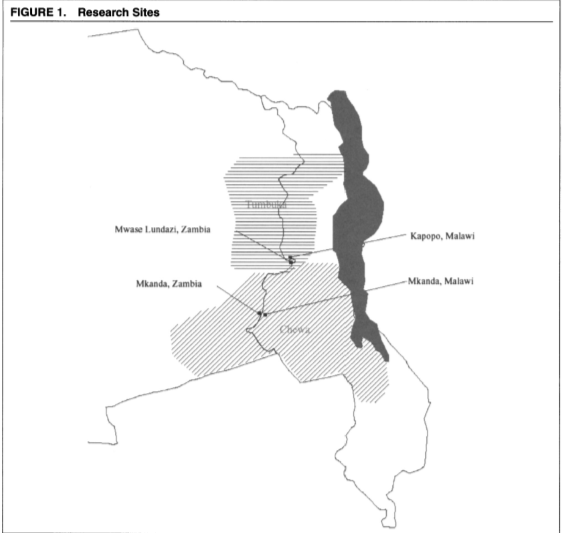
\includegraphics[width=0.9\textwidth]{Posner_map.png}
\end{frame}

\begin{frame}
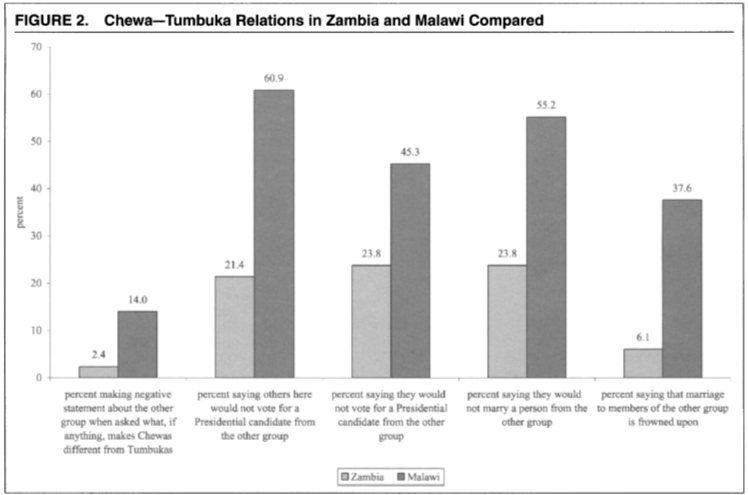
\includegraphics[width=1\textwidth]{Posner_results.png}
\end{frame}

\begin{frame}
\frametitle{Posner (2004)}
\begin{itemize}
\item What is treatment here? \pause Being in Zambia/Malawi
\pause 
\item What is Posner interested in? \pause Large ethnic groups relative to country size
\pause
\item But lots of things are different about Zambia!
\pause
\item Eg. Zambia is \textit{much} richer than Malawi due to copper revenues - maybe politics doesn't need to be as conflictual
\end{itemize}
\end{frame}

\end{document}


%%% Mention SUTVA

%%% Put example of rain 4th july paper... How would you identify effect of independence day marches on national pride?

%%% Emphasis can be only component of treatment that is as-if randomly assigned

%%% Drunken bombings as example of non-random assignment (Lyall). Ask Qs about this.
